\documentclass[a4paper,12pt]{extreport}
\usepackage{capston}


\begin{document}

\onehalfspacing % Set line spacing to 1.5
\justifying % Justify tex
\centering
\logo \\[3em]
\textbf{\LARGE \universityname} \\[1em]
\textbf{\Large \facultyname} \\[1em]
\textbf{\large \departmentname} \\[3em]
\textbf{\Huge \projecttitle} \\[2em]
\textbf{\Large By} \\[1em]
\begin{tabular}[pos]{c} 
    \textbf{\uppercase{hashem vaseghi}}      \\[0.5em] 
    \textbf{\uppercase{Parfait Zaina Ngoi}}  \\[0.5em]
    \textbf{\uppercase{Felly Ngoy}}          \\[0.5em]
    \textbf{\uppercase{Jude Kabemba}}        \\[0.5em]
    \textbf{\uppercase{Boima Fahnbulleh}}   \\[0.5em]
    \textbf{\uppercase{Gregory Mwema}}     \\[0.5em]
    \textbf{\uppercase{Olutoye Opeyemi}}   \\[0.5em]
\end{tabular}
\vfill
\textbf{ Date: \reportdate} \\[1em]
\textbf{ Place: \reportplace} \\[1em]
%this is table of content
\pagenumbering{gobble}

\newpage

\centering
\logo \\[3em]
\textbf{\LARGE \universityname} \\[1em]
\textbf{\Large \facultyname} \\[1em]
\textbf{\large \departmentname} \\[3em]
\textbf{\Huge \projecttitle} \\[2em]
\textbf{\Large By} \\[1em]
\begin{tabular}[pos]{c} 
    \textbf{\uppercase{hashem vaseghi}}      \\[0.5em]
    \textbf{\uppercase{Parfait Zaina Ngoi}}  \\ [0.5em]
    \textbf{\uppercase{Felly Ngoy}}          \\ [0.5em] 
    \textbf{\uppercase{Jude Kabemba}}        \\ [0.5em]
    \textbf{\uppercase{Boima Fahnbulleh}}   \\[0.5em]
    \textbf{\uppercase{Gregory Mwema}}     \\[0.5em]
    \textbf{\uppercase{Olutoye Opeyemi}}   \\[0.5em]
\end{tabular}
\vfill
\textbf{ Date: \reportdate} \\[1em]
\textbf{ Place: \reportplace} \\[1em]
%this is table of content

\newpage

\centering
\textbf{\LARGE \projecttitle} \\[1em]

\textbf{\Large By} \\[3em]
\begin{tabular}[pos]{c c c} \hline
    Hashem Vaseghi     & 22004087 & Electrical and Electronic Engineering \\ 
    Parfait Zaina Ngoi & 22015208 & Electrical and Electronic Engineering \\
    Felly Ngoy         &22013357& Computer Engineering \\
    Jude Kabemba       &22013160& Computer Engineering \\
    Boima Fahnbulleh  & 22013081 & Mechatronics Engineering \\
    Gregory Mwema    & 22012501& Mechatronics Engineering \\
    Olutoye Opeyemi  &22013786& Mechanical Engineering \\
\end{tabular}\\[10em]
{\raggedright
\textbf{DATE OF APPROVAL: ................}\\[2em]
APPROVED BY: \\[4em]
\textbf{\supe} \\[2em]
{\raggedleft
\textbf{ \rule{5cm}{0.4pt} }\\[7em]}
\textbf{\supm} \\[2em]
{\raggedleft
\textbf{ \rule{5cm}{0.4pt} }\\[2em]}
\vfill
%this is table of content
}
\newpage

\pagenumbering{Roman}
\centering
\section*{ACKNOWLEDGEMENTS}
\justifying % Justify text
We extend our heartfelt appreciation to everyone who contributed to the success of this project. First and foremost, we express our deepest gratitude to \textbf{Asst. Prof. Dr. ZİYA DEREBOYLU} and \textbf{Asst. Prof. Dr. ALİ SHEFIK} for their invaluable guidance, continuous support, and encouragement throughout the project. Their expertise and insights were instrumental in overcoming challenges and ensuring the project's progress.

We are also grateful to \textbf{Cyprus International University} for providing us with the resources and platform to pursue this project. Special thanks to the faculty members of the \textbf{Faculty of Engineering} for their technical advice and mentorship, which greatly enriched our learning experience.

Our sincere thanks go to our entire team for their dedication and collaboration. Each member brought unique skills and perspectives, contributing to the successful integration of mechanical, electronic, and software systems. This project would not have been possible without their united commitment and hard work.

We also extend our gratitude to our families and friends for their unwavering support, encouragement, and motivation during the challenging phases of the project.

Finally, we would like to thank the organizers of the Teknofest Aerospace and Technology Festival for providing us with the opportunity to showcase our work and compete in the Digital Technologies in Industry competition.

This project is a testament to the collective effort and support of everyone involved. Thank you all for being part of this journey.
\newpage
\centering
\section*{ABSTRACT}
\justifying
The research introduces CIU\_Fox as an autonomous guided vehicle (AGV) that develops capabilities to transform factory and warehouse internal transportation operations. The designed AGV features autonomous navigation with a safe lifting capability using obstacle detection and collision avoidance systems for moving loads up to 200 kg.
This system combines LIDAR with time-of-flight (ToF) sensors and barcode scanners to create a precise automated navigation system which monitors operations and handles loading duties.
The mechanical structure incorporates an aluminum alloy frame together with a scissor-compartment mechanism and NEMA 23 stepper-motor powered differential steering.
A Raspberry Pi 4 manages the system through ESP32 modules that run software programs built in Python and C++ within the ROS framework.
The robot development followed four sequential stages that led to its physical assembly. Resources limitations required the project team to conduct final stage testing through the Gazebo simulation pipeline instead of building physical components. Coding for path planning alongside obstacle avoidance and load management functions while achieving complete integration of mechanical electronic software system components stands as major accomplishments. The commercial application scope of the AGV remains promising in multiple industrial sectors including manufacturing storage facilities and logistics operations because it shows potential to optimize operational efficiency while decreasing expenses and protecting worker safety.  
This work illustrates why interdisciplinary teams need to bring innovative solutions to modern industrial design using state-of-the-art technology applications. Research efforts will focus simultaneously on two fronts which include enhancing the AGV's operational excellence while evaluating opportunities to connect it with broader industrial system networks.
\newpage

\centering
\tableofcontents
\newpage

\listoffigures
\newpage

\listoftables
\newpage
%nex page is the report
\pagenumbering{arabic}
\justifying
\chapter{introduction}

Today’s industries activity have merged
with the robotic and automation world and
day by day having the precise and betterquality
product make the sense of using
new technology. Between all types of
robot, the AGV (automated guided
vehicle) robot has the special place
between others and improvement in
technology helps this design to grow and
become more helpful in various
applications. The AGV robot is a
programmable mobile robot integrated
sensor device that can automatically
perceive and move along the planned
path\cite{das2016design} This system consists of various
parts like guidance facilities, central
control system, charge system and
communication system\cite{moshayedi2019agv}. 

The initial used and Invention AGV is not clear exactly and
was mentioned in different articles and
reference for many times but the earliest
time of using this system in industries is
mentioned in 1950s \cite{reveliotis2000conflict}
(\cref{oldAgv}) and even
mentioned in some reference that the first
AGV in the world was introduced in UK in
1953 for transporting which was modified
from a towing tractor and can be guided by
an overhead wire \cite{moshayedi2019agv}.

\begin{figure}[H]
    \centering
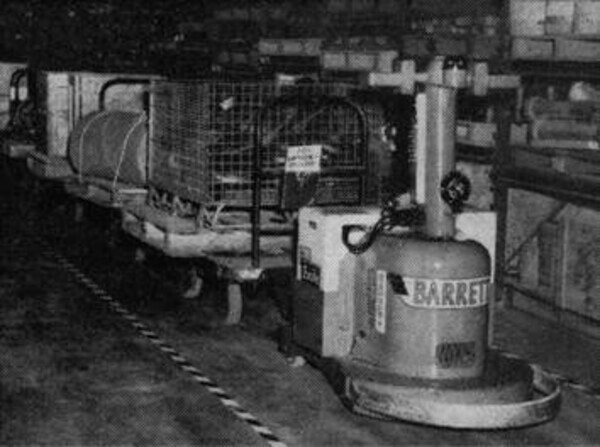
\includegraphics[width=0.5\textwidth]{doc/oldestAGV.jpg}
\caption{one of the Old AGV picture}
\label{oldAgv} % Unique label for referencing
\end{figure}

AGVs are widely applied in various kinds
of industries including manufacturing
factories and repositories for materialhandling.
After decades of development, it
has a wide application due to its high
efficiency, flexibility, reliability, safety and
system scalability in various task and
missions.
AGV operates all day long continuously
that cannot be achieved by human workers.
Therefore, the efficiency of material
handling can be boosted by having the
collaborating task with number of AGV
. In this case, administrator can enable
more AGVs as the system is extensible.
AGV has capability of collision avoidance
and emergency braking, and generally the
running status is monitored by control
system so that reliability and safety are
ensured. Generally, a group of AGVs are
monitored and scheduled by a central
control system. AGVs, ground navigation
system, charge system, safety system,
communication system and console make
up an AGV system. \cite{shengfang2006research}. This report examines the design aspects and considerations for this type of robot, providing readers with key insights into the technologies commonly utilized in this field. 


\newpage
\chapter{Theory of AGV Design}
\begin{figure}[h]
    \centering
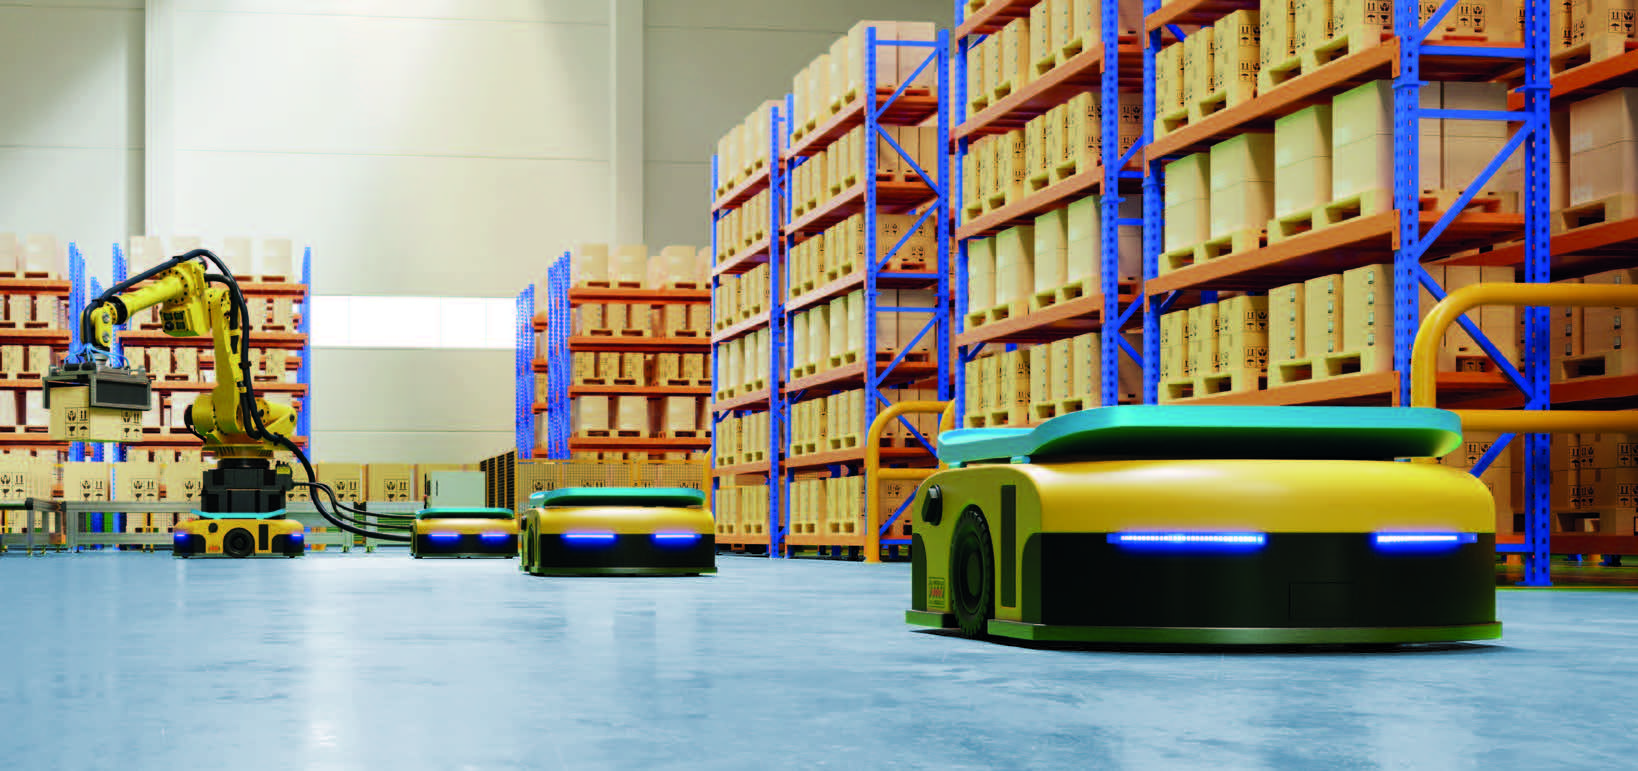
\includegraphics[width=\textwidth]{doc/smart_agv.jpg}
\caption{Smart AGV in Industry 4.0}
\end{figure}
AGVs are essential components in modern industrial automation systems, designed to improve efficiency, flexibility, and safety in material handling and logistics. This section discusses the fundamental theories and principles underlying AGV design, including navigation, control, and system integration.



%\chapter{REALISTIC CONSTRAINTS }

\subfileinclude{sublatex/hashem/ROS}
\subfileinclude{sublatex/hashem/urdf}
\subfileinclude{sublatex/felly/felly}
\subfileinclude{sublatex/Opryrmi/Opryrmi}

%%Must be include: Formulation,
%and solution of the necessary
%engineering problems for their project;
%selection and application to proper 
%analysis and modeling methods for 
%their project. Use theoretical and 
%applied knowledge for their project.
%%%%%%%%%%%%%%%%%%%%%%%%%%%%%%%%%%%%%%%%%%%%%%%%%%%%%%%%%%%%%%%
\newpage
\chapter{METHODS USED TO DESIGN THE PROJECT }

%%%%%%%%%%%%%%%%%%%%%%%%%%%%%%%%%%%%%%%%%%%%%%%%%%%%%%%%%%%%%%%
\newpage
\chapter{CONCLUSION AND FUTURE WORKS}

\section{COST}
\begin{longtable}{|m{5cm}|c|c|m{3cm}|}
    
    \caption{here is the list of components}\\
    \hline
    Components & Quantity & Price(per Unit)& ref \endfirsthead  \hline \hline
    Raspberry Pi 4 8GB RAM &1 &3127.03 \faTry  &\includegraphics*[width=3cm, height=2cm]{compont/rasp.png} \\ \hline
    ESP32-S3-DevKitC-1-N8R8 - ESP32-S3-WROOM-1 &2 &1220 \faTry & \includegraphics*[width=2.5cm, height=2cm]{compont/esp32.png}\\ \hline
    Closed Loop Stepper Driver V4.1 0-8.0A 24-48VDC CL57T &2 &1186 \faTry &\includegraphics*[width=2.5cm, height=2cm]{compont/Clsd-Lood-Drive.png}\\ \hline
    Motorobit Weight Sensor 120 kg &2 &768.2 \faTry  &\includegraphics*[width=2.5cm, height=2cm]{compont/Ws120.png}\\ \hline
    Weight Sensor - Load Sensor 50Kg. &4 &29.7 \faTry &\includegraphics*[width=2.5cm, height=2cm]{compont/Ws50.png}\\ \hline
    Load Cell Amplifier - HX711 & 4&27.3 \faTry &\includegraphics*[width=2.5cm, height=2cm]{compont/Loadeh711.png}\\ \hline
        BTS7960B 40 Amp Motor Driver Board &1 &188.82 \faTry &\includegraphics*[width=2.5cm, height=2cm]{compont/BTS-Driver.png}\\ \hline
        Barcode Scanner Module 1D/2D Codes Reader & 1&1261.83 \faTry &\includegraphics*[width=2.5cm, height=2cm]{compont/barcode.png}\\ \hline
        QTRXL-MD-01A Reflectance Sensor Array &4 &90.57 \faTry &\includegraphics*[width=2.5cm, height=2cm]{compont/QTRX.png}\\ \hline
        Gravity: HUSKYLENS &1 &1723.14 \faTry &\includegraphics*[width=2.5cm, height=2cm]{compont/Husky.png}\\ \hline
        IMU Sensor / 9 Axis MPU9255 IMU and Barometric Sensor (Low Power) &1 &1058.31 \faTry &\includegraphics*[width=2.5cm, height=2cm]{compont/IMU.png} \\ \hline
        RPLIDAR - 360 degree Laser Scanner Development Kit &1 &5029.72 \faTry &\includegraphics*[width=2.5cm, height=2cm]{compont/LIDAR.png} \\ \hline
        TXS0108E 8 Channel Voltage Level Transducer &4 &40 \faTry & \includegraphics*[width=2.5cm, height=2cm]{compont/voltageShifter.png} \\ \hline
        The VL53L0X is a time-of-flight (ToF) distance sensor &10 &101.76 \faTry &\includegraphics*[width=2.5cm, height=2cm]{compont/TOF.png}\\ \hline
        UV Solder Mask  &3 &180.78 \faTry &\includegraphics*[width=2.5cm, height=2cm]{compont/UV-soldir.png}\\ \hline
        LM2596HV/LM2576 Voltage Regulator for Multiple power supply   &4 &36.09 \faTry &\includegraphics*[width=2.5cm, height=2cm]{compont/5vregulator.png}\\ \hline
        Aluminum heatsink  &2 &439 \faTry &\includegraphics*[width=2.5cm, height=2cm]{compont/heatSinc.png}\\ \hline
        5V 8 Channel Relay Card  &1&154.68 \faTry &\includegraphics*[width=2.5cm, height=2cm]{compont/relay.png} \\ \hline
        P Series Nema 23 Closed Loop Stepper Motor 2Nm(283.28oz.in) with Electromagnetic Brake  & 2&2971.78 \faTry &\includegraphics*[width=2.5cm, height=2cm]{compont/mainMotor.png}\\ \hline
        EG Series Planetary Gearbox Gear Ratio 20:1 Backlash 20arc-min for 10mm Shaft Nema 23 Stepper Motor  &2 &1642 \faTry &\includegraphics*[width=2.5cm, height=2cm]{compont/gearBox.png} \\ \hline
        Shaft Sleeve Adaptor 11mm to 8mm for NMRV30 Worm Gearbox  &4 &35 \faTry &\includegraphics*[width=2.5cm, height=2cm]{compont/11to8Adaptor.png}\\ \hline
        Single Output Shaft for NMRV30 Worm Gearbox  &4 &121.37 \faTry &\includegraphics*[width=2.5cm, height=2cm]{compont/Worm-GearBox.png}\\ \hline
        Double Output Shaft for NMRV30 Worm Gearbox  &4 &121.37 \faTry &\includegraphics*[width=2.5cm, height=2cm]{compont/Worm-GearBox.png}\\ \hline
        NEMA 23 Stepper Motor Vibration Damper  &4 &243.74 \faTry &\includegraphics*[width=2.5cm, height=2cm]{compont/Damper.png}\\ \hline
        Nema 23 Bracket for Stepper Motor  &4 &243.74 \faTry &\includegraphics*[width=2.5cm, height=2cm]{compont/bracket-motor.png}\\ \hline
        Nema 23 Flange for ISC And ISD Series Drivers  &3 &175.28 \faTry &\includegraphics*[width=2.5cm, height=2cm]{compont/Flang.png}\\ \hline
        AWG  20 High-flexible with Shield Layer Stepper Motor Cable  &2 &43.25 \faTry &\includegraphics*[width=2.5cm, height=2cm]{compont/motor-cable.png}\\ \hline
        TP-Link TL-WR840N  &1 &569 \faTry &\includegraphics*[width=2.5cm, height=2cm]{compont/TP-link.png}\\ \hline
        Raspberry Pi 4.3 Inch Capacitive Touch Screen DSI Interface 800"480  &1 &1750.28 \faTry &\includegraphics*[width=2.5cm, height=2cm]{compont/raspb-LCD.png}\\ \hline
        Nema 8R 5W 87dB 90X39mm Speaker  &1 &108.11 \faTry &\includegraphics*[width=2.5cm, height=2cm]{compont/speaker.png}\\ \hline
        Nema RS232 to Bluetooth Series Adapter  &2 &455 \faTry &\includegraphics*[width=2.5cm, height=2cm]{compont/BLU-Adaptor.png}\\ \hline
        12V 70 AH AGM BATTERY   &1 &5000 \faTry &\includegraphics*[width=2.5cm, height=2cm]{compont/battery.png}\\ \hline
        Battery Chargers 6V/2A 12V/2A Full Automatic Smart Battery  &1 &642.99 \faTry &\includegraphics*[width=2.5cm, height=2cm]{compont/charger.png}\\ \hline
        RS232 Adapter Cable to USB 2.0  & 2&453.65 \faTry &\includegraphics*[width=2.5cm, height=2cm]{compont/EX1.png}\\ \hline
        Motor and encoder extension cable kit &2 &351 \faTry &\includegraphics*[width=2.5cm, height=2cm]{compont/EX2.png}\\ \hline
        DC 12V Electric Linear Actuator Force 6000N  &1 &2479 \faTry &\includegraphics*[width=2.5cm, height=2cm]{compont/LinearAC.png}\\ \hline
        WM-045 DC-DC 150W Voltage Booster &1 &521.04 \faTry &\includegraphics*[width=2.5cm, height=2cm]{compont/150W.png}\\ \hline
        Motorobit DC-DC 1500W 30A Voltage Boost Module &1 & 881.76 \faTry&\includegraphics*[width=2.5cm, height=2cm]{compont/1500W.png}\\ \hline
        TCA9548A I2C Çoklayıcı / Multiplexer Kartı &1 &40.66 \faTry &\includegraphics*[width=2.5cm, height=2cm]{compont/multiplexer.png}\\ \hline
        3B Printer Limit Switch & 2&37.07 \faTry &\includegraphics*[width=2.5cm, height=2cm]{compont/LimitSW.png}\\ \hline
        Drn956 16mm Acil - Stop Switch (Kafa 27mm) & 1&145.08 \faTry &\includegraphics*[width=2.5cm, height=2cm]{compont/stopeSW.png}\\ \hline
        
        
    
\end{longtable}
%%%%%%%%%%%%%%%%%%%%%%%%%%%%%%%%%%%%%%%%%%%%%%%%%%%%%%%%%%%%%%%
\newpage
\chapter*{APPENDIX}

%%%%%%%%%%%%%%%%%%%%%%%%%%%%%%%%%%%%%%%%%%%%%%%%%%%%%%%%%%%%%%%
%\newpage
%\chapter*{REFERENCES}

\bibliography{references}

\end{document}


